% !TEX root = ../../main.tex

\subsection{Pattern Selection Validation}

The previous sections evaluated OTFS-IM as an end-to-end transmission scheme. This section focuses on the pattern-selection component itself. In the proposed OTFS-IM transmitter, only a subset of all possible activation patterns is used for mapping the index bits. The purpose of OHD and B-OHD selection is to choose this subset more carefully than a purely arbitrary pattern table. The validation therefore compares deterministic pattern selection with a random-pattern diagnostic baseline.

The configuration \(n=5,k=3\) is used as the main validation case because it provides a non-trivial pattern-selection problem while keeping the exact OHD search feasible. For this configuration, there are \(\binom{5}{3}=10\) possible constant-weight activation patterns, and the system selects \(2^{b_1}=8\) patterns for index-bit mapping. Hence, OHD and B-OHD are forced to discard some candidate patterns, but the candidate set is still small enough to allow an exact comparison. This makes the configuration suitable for explaining the effect of pattern geometry without making the pattern-selection result visually or computationally excessive.

\IfFileExists{Images/Chapter5/pattern_geometry_n5_k3.png}{%
\begin{figure}[H]
    \centering
    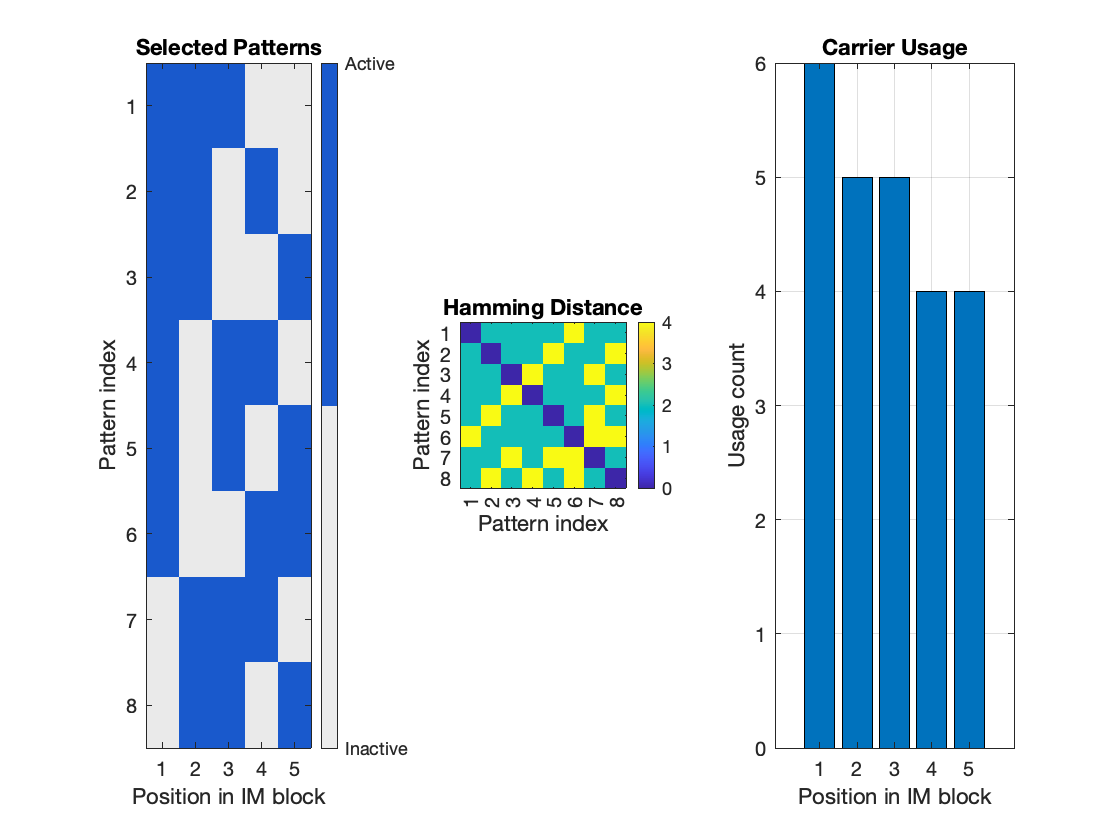
\includegraphics[width=0.92\linewidth]{Images/Chapter5/pattern_geometry_n5_k3.png}
    \caption{Selected pattern geometry for OHD-based OTFS-IM with \(n=5,k=3\)}
    \label{fig:chapter5_pattern_geometry_n5_k3}
\end{figure}
}{%
\begin{figure}[H]
    \centering
    \fbox{%
        \begin{minipage}[c][0.25\textheight][c]{0.88\linewidth}
            \centering
            Required figure file is missing:\\
            Images/Chapter5/pattern\_geometry\_n5\_k3.png
        \end{minipage}
    }
    \caption{Selected pattern geometry for OHD-based OTFS-IM with \(n=5,k=3\)}
    \label{fig:chapter5_pattern_geometry_n5_k3}
\end{figure}
}

Figure~\ref{fig:chapter5_pattern_geometry_n5_k3} illustrates the selected activation patterns and their geometric properties. The selected-pattern map shows which positions are active in each IM block. The Hamming-distance map indicates how different the selected patterns are from each other, while the carrier-usage plot shows whether the active positions are distributed evenly across the block. These three views are useful because pattern selection in OTFS-IM is not only about maximizing pairwise distance. A pattern table with good distance but unbalanced carrier usage may still create unequal position reliability.

For the \(n=5,k=3\) configuration, the spectral efficiency is
\begin{equation}
    \eta_{\mathrm{IM}}
    =
    \frac{\left\lfloor \log_2 \binom{5}{3} \right\rfloor + 3\log_2 4}{5}
    =
    \frac{3+6}{5}
    =
    1.80~\text{bits/symbol}.
    \label{eq:chapter5_se_53_validation}
\end{equation}
This rate is lower than the baseline OTFS rate of \(2.00~\text{bits/symbol}\), so this configuration should be interpreted as a reliability-oriented OTFS-IM setting rather than a strict equal-SE comparison. The BER improvement obtained in this case therefore represents a BER-SE trade-off: the system sacrifices \(10\%\) spectral efficiency to improve reliability in the medium-to-high-SNR region.

The geometry result also explains the difference between OHD and B-OHD. With OHD, the selected pattern table has carrier usage \([6,5,5,4,4]\), which indicates that the first position is activated more often than the last two positions. B-OHD preserves the same minimum Hamming distance but improves the usage balance to approximately \([5,4,5,5,5]\). This does not change the basic OTFS-IM structure, but it makes the selected pattern table less biased toward a small number of positions. Such balancing is expected to be more useful when the detector output is already reliable enough for the remaining pattern-geometry differences to matter.

\IfFileExists{Images/Chapter5/pattern_validation_n5_k3.png}{%
\begin{figure}[H]
    \centering
    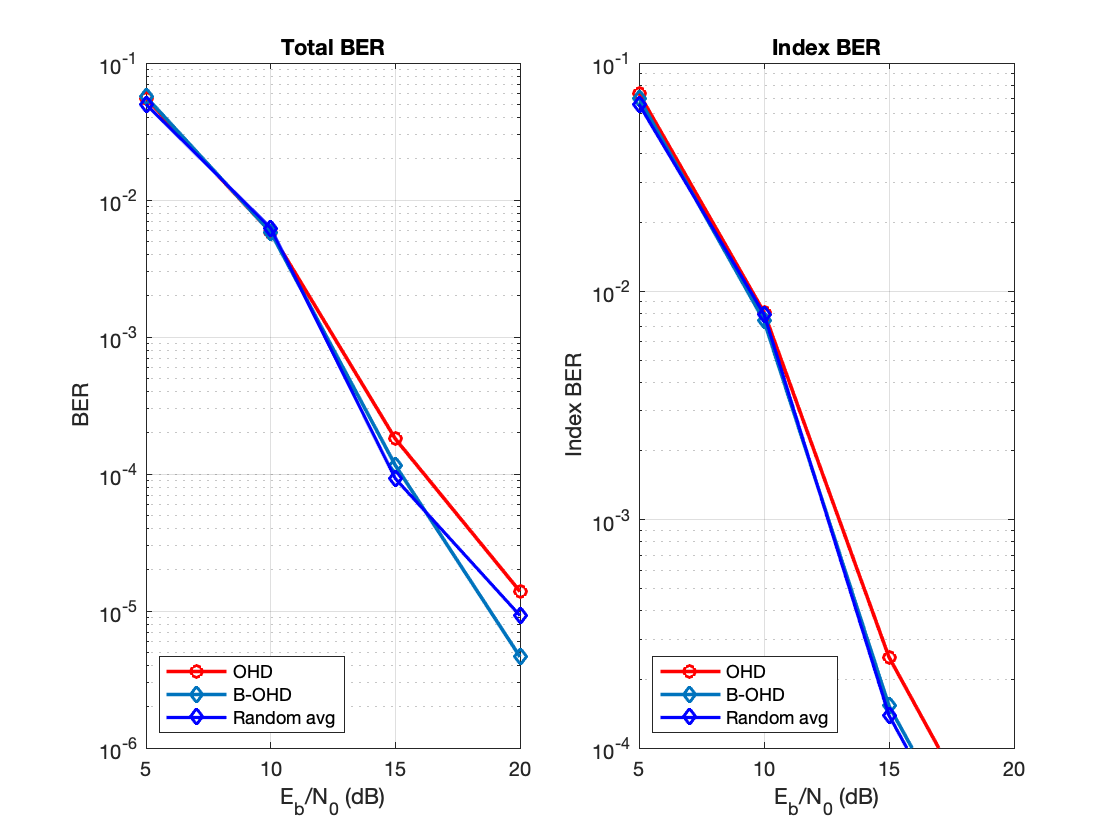
\includegraphics[width=0.95\linewidth]{Images/Chapter5/pattern_validation_n5_k3.png}
    \caption{Validation of OHD and B-OHD pattern selection against random pattern tables for \(n=5,k=3\)}
    \label{fig:chapter5_pattern_validation_n5_k3}
\end{figure}
}{%
\begin{figure}[H]
    \centering
    \fbox{%
        \begin{minipage}[c][0.28\textheight][c]{0.88\linewidth}
            \centering
            Required figure file is missing:\\
            Images/Chapter5/pattern\_validation\_n5\_k3.png
        \end{minipage}
    }
    \caption{Validation of OHD and B-OHD pattern selection against random pattern tables for \(n=5,k=3\)}
    \label{fig:chapter5_pattern_validation_n5_k3}
\end{figure}
}

Figure~\ref{fig:chapter5_pattern_validation_n5_k3} compares OHD, B-OHD, and the random-pattern average. The random curve is not used as a proposed design method in this thesis. Instead, it is used as a diagnostic reference to check whether the deterministic selection rules provide a meaningful advantage over arbitrary pattern choices. This comparison is necessary because a random pattern table can sometimes have favorable distance or usage properties, especially when the candidate set is small.

At \(10~\mathrm{dB}\), the total BER values are approximately \(5.81\times10^{-3}\), \(5.81\times10^{-3}\), and \(6.24\times10^{-3}\) for OHD, B-OHD, and random selection, respectively. At this SNR point, deterministic pattern selection provides a modest but visible improvement over the random average. The index BER values are also close: \(8.10\times10^{-3}\) for OHD, \(7.43\times10^{-3}\) for B-OHD, and \(7.94\times10^{-3}\) for the random average. This indicates that B-OHD slightly improves the index reliability compared with OHD while remaining competitive with the random baseline.

At \(15~\mathrm{dB}\), the performance difference becomes more visible in the total BER. OHD reaches approximately \(1.81\times10^{-4}\), B-OHD reaches \(1.16\times10^{-4}\), and the random average reaches \(9.0\times10^{-5}\). The random average is slightly lower at this point, but B-OHD still improves over the original OHD table. This result should not be interpreted as a failure of deterministic pattern selection. Rather, it shows that random pattern tables can occasionally be strong, and that the proposed deterministic design should be evaluated against them instead of only against the OTFS baseline.

The pattern error rate provides an additional explanation. At \(10~\mathrm{dB}\), the pattern error rates are approximately \(1.47\times10^{-2}\), \(1.36\times10^{-2}\), and \(1.49\times10^{-2}\) for OHD, B-OHD, and random selection, respectively. B-OHD gives the lowest pattern error rate in this region, which is consistent with its improved carrier-usage balance. At \(15~\mathrm{dB}\), all three methods have very small pattern error rates, and the remaining BER differences become sensitive to both symbol decisions and Monte Carlo variation.

Overall, the \(n=5,k=3\) validation gives a clearer pattern-selection story than configurations where OHD and B-OHD overlap. OHD provides a structured pattern table based on Hamming-distance separation, while B-OHD improves the balance of the selected table without changing the OTFS-IM receiver. The results show that B-OHD can improve OHD, especially in the medium-to-high-SNR region. At the same time, the random baseline remains important because it shows that pattern selection is configuration-dependent and that Hamming distance alone does not guarantee universal superiority. This observation motivates future channel-aware or detector-aware pattern selection methods, while still supporting the use of structured pattern design in the present OTFS-IM system.
